

\documentclass{article}
\usepackage{graphicx} % for figures
\usepackage{float}
\usepackage[export]{adjustbox}
\usepackage{fancyhdr}
\begin{document}

\title{Physics 240 - Final Project\\
		Roche surfaces}
\author{Tin Tran}

\maketitle

\section{Introduction}
The topic of my project is computing the Roche surfaces of a system of binary stars. I chose this topic because I think it's an interesting Astronomy topic and it's a good way to practice what we've been learning in class regarding all the plotting and computation methods.\\
A littel bit of bacgkground. The effect grativational potential of two bodies orbiting each other in the x-y plane is given by:
\begin{center}
V(x,y) = -G$\frac{M_1}{r_1}$ - -G$\frac{M_2}{r_2}$ - $\omega^2\frac{x^2+y^2}{2}$
\end{center}
This is a co-rotating coordinate system. M$_1$ is at position a on the x-axis and M$_2$ is locate at position -b on the x-axis. The origin is the center of mass and the positions of the 2 stars are:
\begin{center}
r$_1$ = $\sqrt{(x-a)^2+y^2}$ and r$_2$ = $\sqrt{(x+b)^2+y^2}$\\
\end{center}
With $\omega^2$ = $\frac{G*(M_1+M_2)}{a^3}$ where a is the distance between 2 stars.\\
The equipotential surfaces of the binary systems are called Roche lobes. A Roche lobe is the region of space around a star in a binary system within which orbiting objects are bound gravitationally to that star. If it's a binary star system, then the objects would fall through the inner Lagrangian points, the region bounded by critical gravitational potential.  My code would solve and plot those Roche Lobes, which show all the Lagrangian points (5 of them) for different set of Binary star Systems. 

\section{Method and Data}
The scope of my project is not as deep as I originially thought it would be. Instead of solving for each of the Lagragian points by solving the equation $\nabla$V = 0, where V is the effective potential of the system. Solving this would give the exact values of the Lagrangian points. Instead, I only need to plot the V potential with the appropriate values for mass, distance, and the contour levels to show all of the Lagrangian points and all the Roche Lobe.

\section{Results}
The first set of the Data is the Earth-moon System. This system has many similarities to a binary star system so I chose it as a starting point. The plots are produced below:
\begin{figure}[H]
\centering{
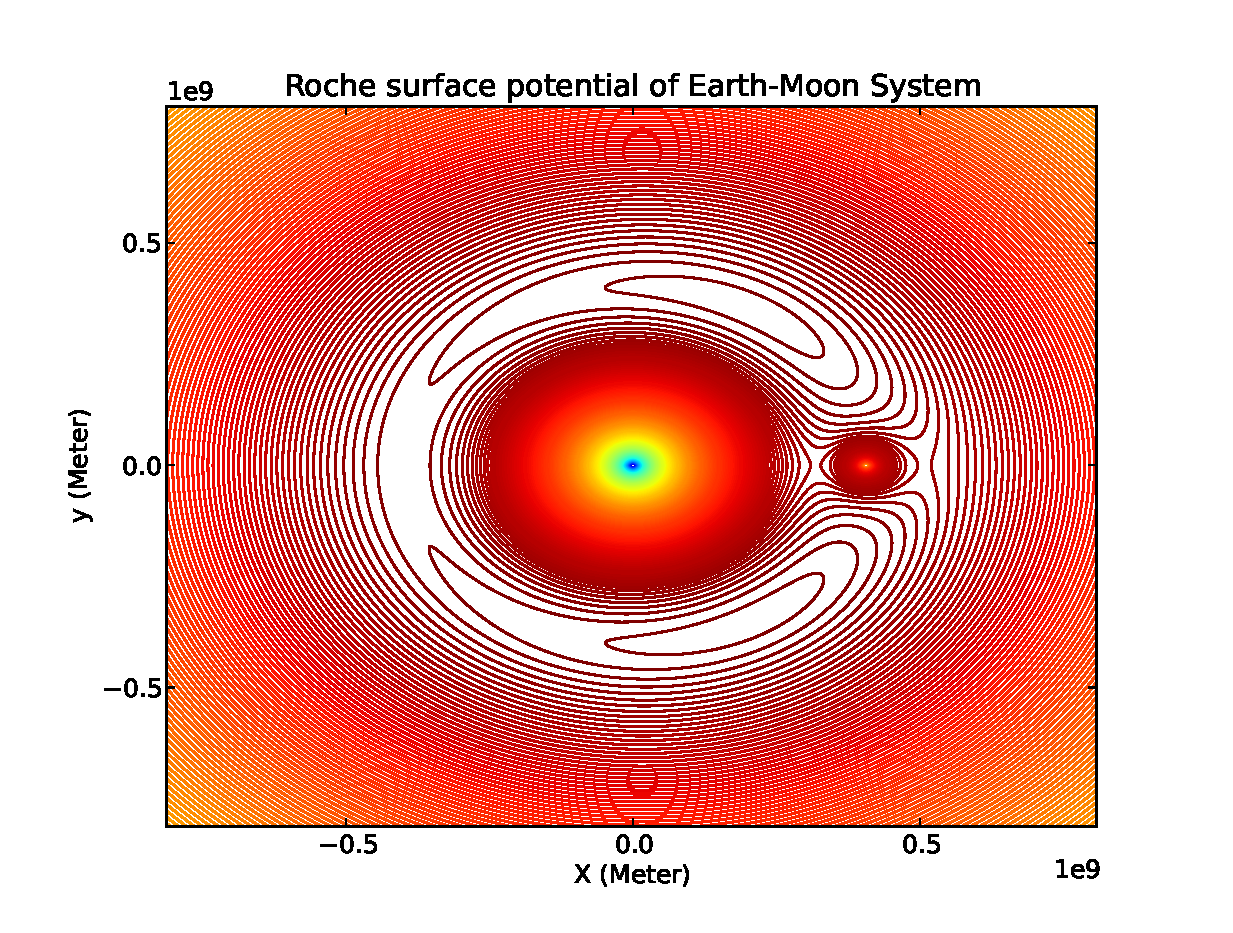
\includegraphics[max size={\textwidth}{\textheight}]{Earthmoon1.eps}
\caption{Roche Lobes of the Earth-Moon System}
}
\end{figure}

\begin{figure}[H]
\centering{
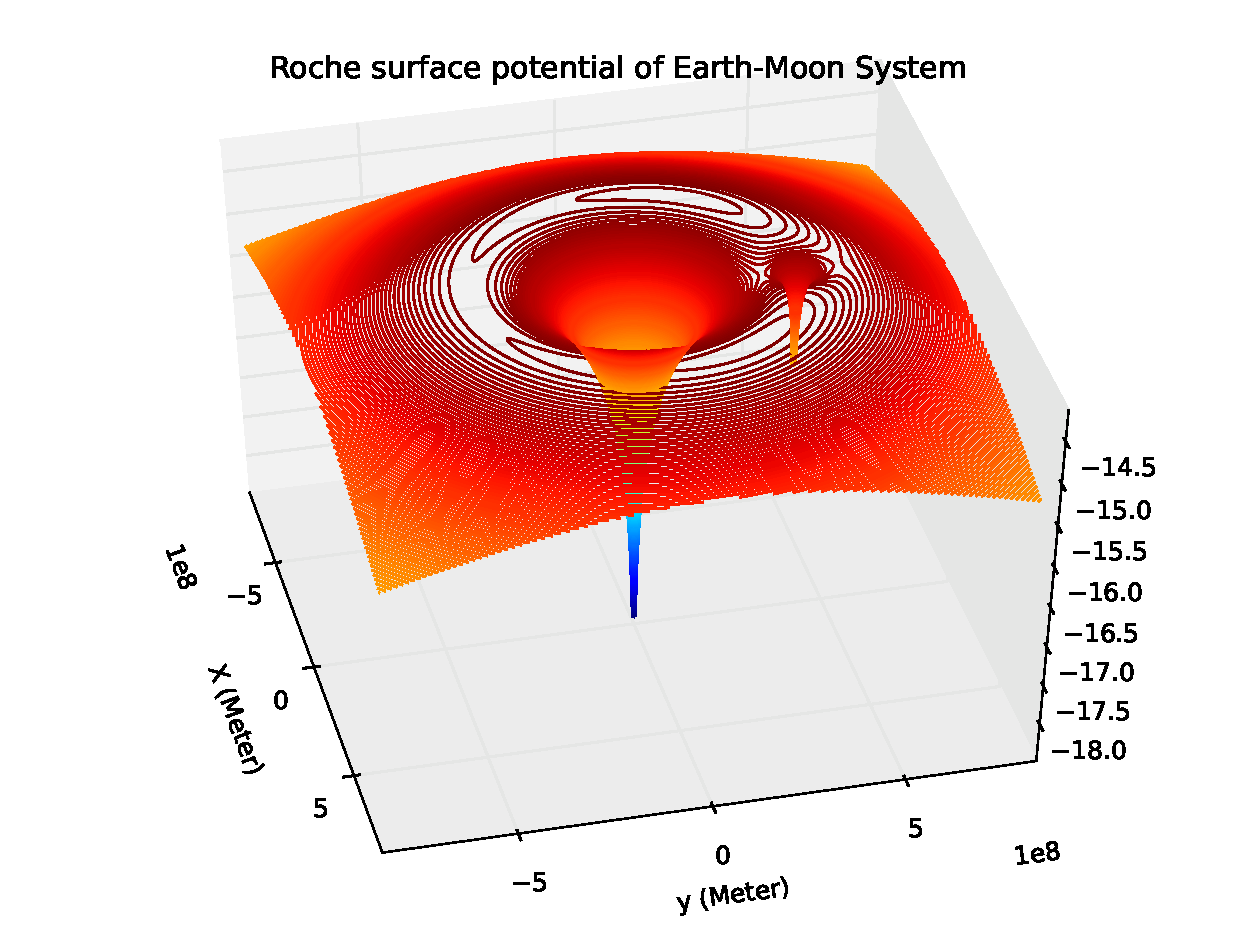
\includegraphics[max size={\textwidth}{\textheight}]{Earthmoon2.eps}
\caption{Roche Lobes of the Earth-Moon system}
}
\end{figure}
For this system, the code didn't work as well as I would have thought. Mainly because the function I have is for binary stars system with their masses less than 1 maginetude of each other. Here, the mass of Earth of 2 magnitudes more than the Mass of the Moon, hence the positions of the Lagrangians isn't well showned here.
\subsection{Binary system Algol}
The next system I computed is the Algol system. The information regarding this system can be found here: http://en.wikipedia.org/wiki/Algol. I choose this star system because it has mass ratio of 2:1, between the 2 Stars. This is a good exampleto see of the Roche Lobes will be different from the Earth-Moon System. The plots are produced below.
\begin{figure}[H]
\centering{
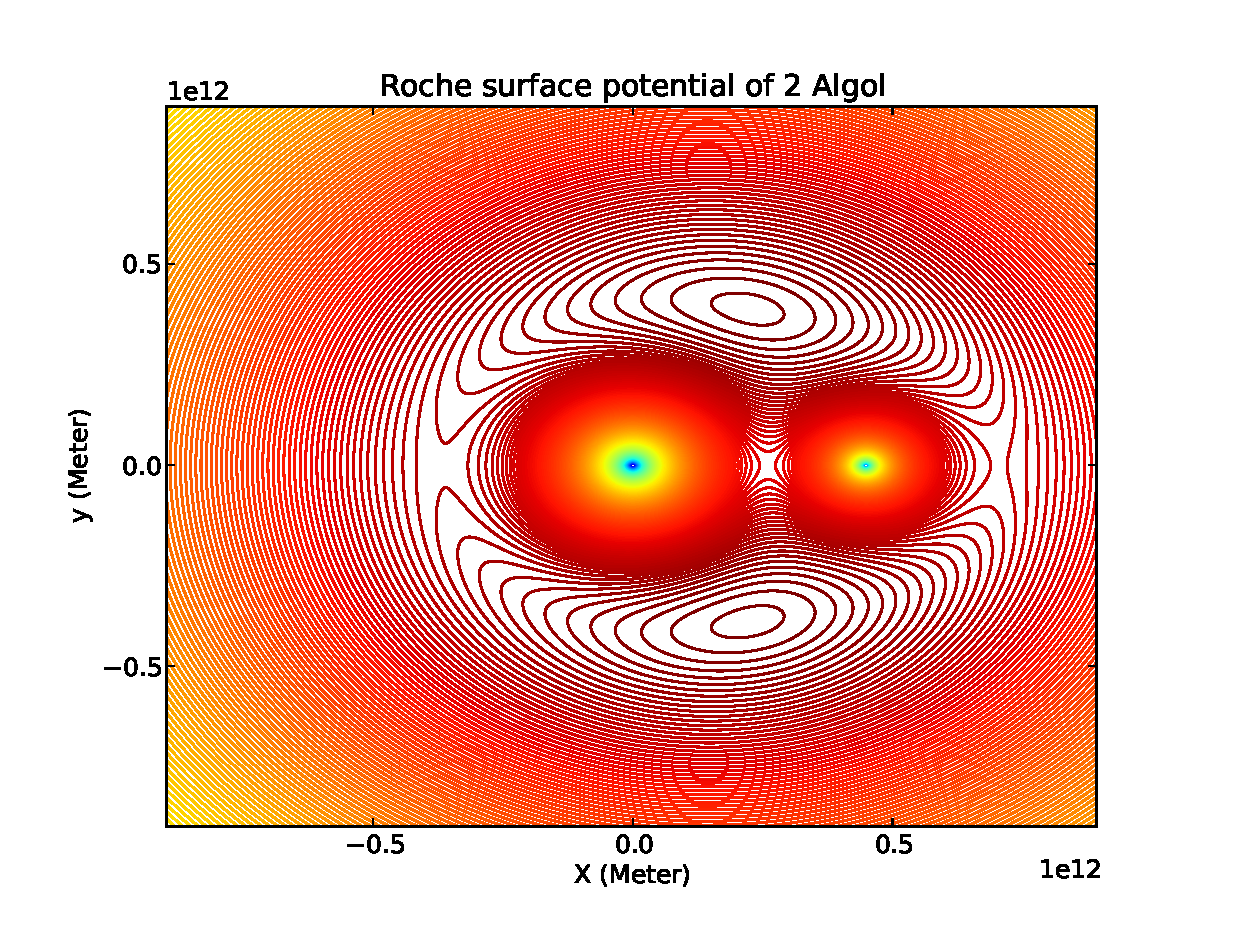
\includegraphics[max size={\textwidth}{\textheight}]{Algol1.eps}
\caption{Roche Lobes of the Algol System}
}
\end{figure}
With this plot, we can clearly see the 5 Lagrangian points, as the mass of the 2 bodies are closer to each other. However, we can also see which one has more mass than the other, and the ratio here is 2.
\begin{figure}[H]
\centering{
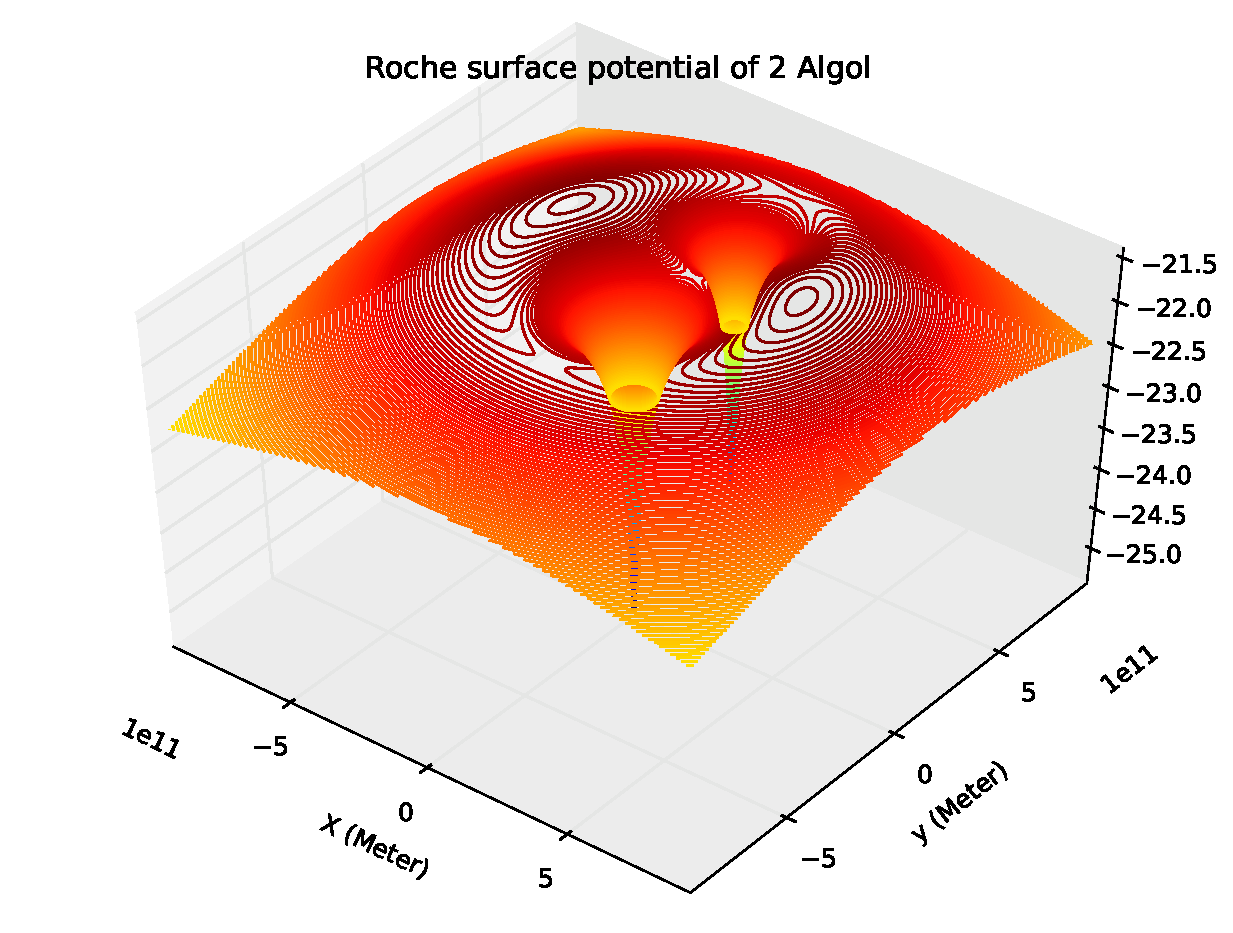
\includegraphics[max size={\textwidth}{\textheight}]{Algol2.eps}
\caption{Roche Lobes of the Earth-Moon system}
}
\end{figure}

\subsection{Binary system Alpha Centauri}
The next system I chose is the Alpha Centauri System. The information regarding this system of which I used can be found here: http://en.wikipedia.org/wiki/Alpha\_Centauri. I chose this system because the mass ratio is 1:1. This is a good example to show how much the Roche lobes wil be different compared to the 2:1 ratio and the Earth-moon system. The plots are produced below.
\begin{figure}[H]
\centering{
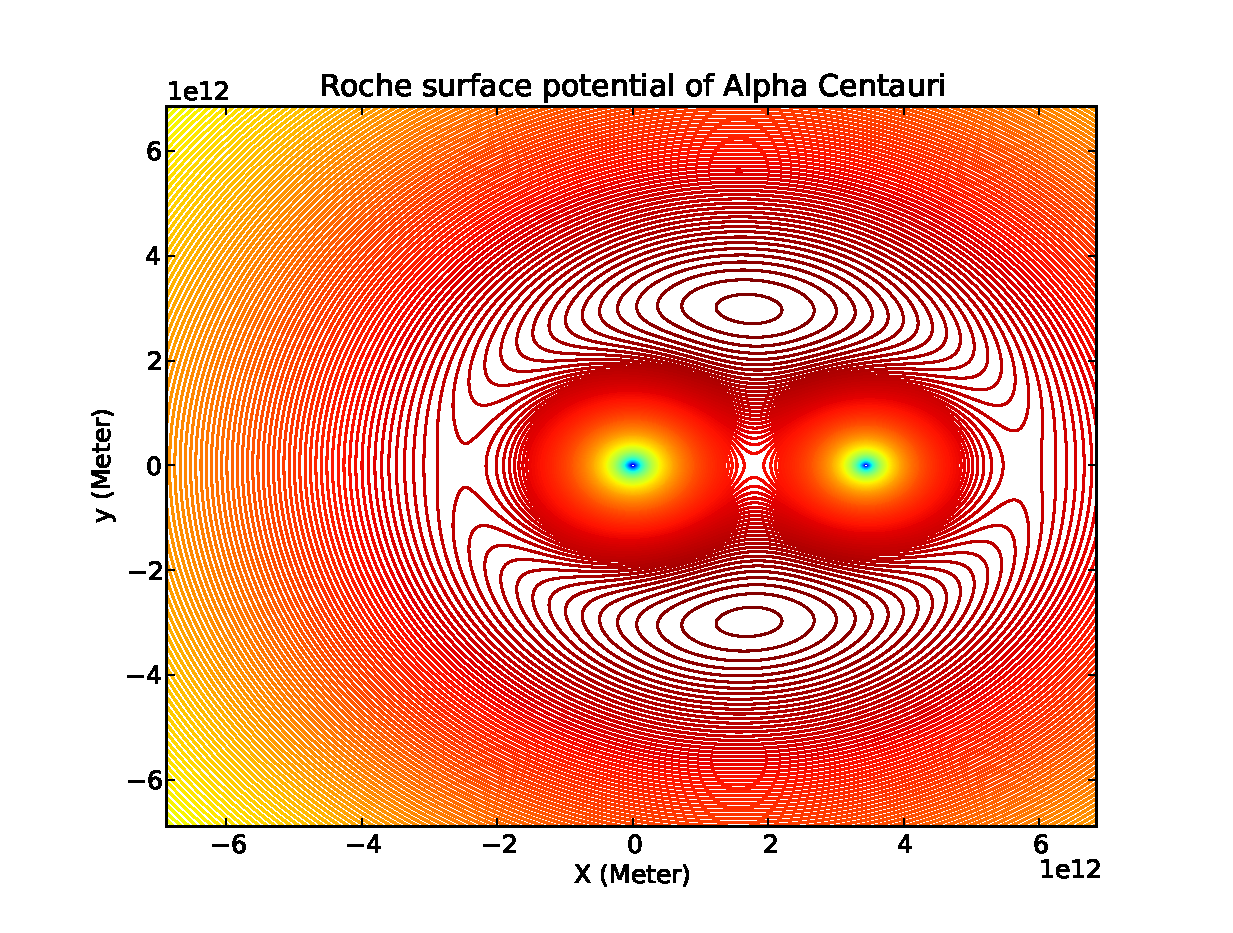
\includegraphics[max size={\textwidth}{\textheight}]{Alpha1.eps}
\caption{Roche Lobes of the Alpha Centauri System}
}
\end{figure}
Similar to the Algol system, we can clearly see the 5 Lagrangian points. The mass ratio is 1:1 and we can clearly see that from the plot.
\begin{figure}[H]
\centering{
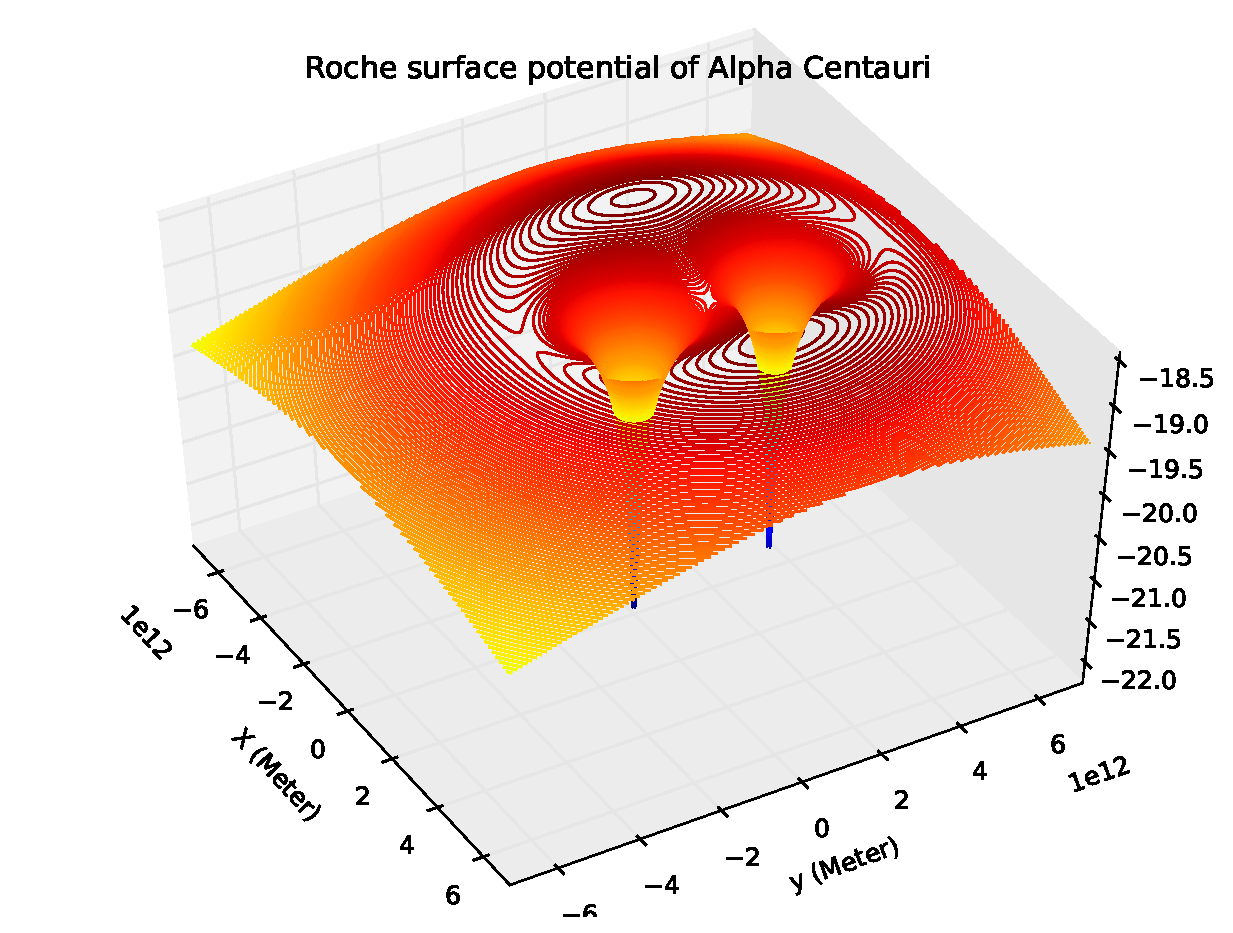
\includegraphics[max size={\textwidth}{\textheight}]{Alpha2.eps}
\caption{Roche Lobes of the Alpha Centauri system}
}
\end{figure}

\section{Summary and After thoughts}
With this project, I have learned a lot regarding contour plots, 3D plots, as well as the computational methods to calculate the positions of the bodies in the system (this is for animation, which I have yet to finish, and hopefully will be finished before the presentation on Tuesday. In my code. I have the option to enter user inputs, which I plan to enter a few more systems to see how they will behave. Overall, this was a fun project and it has helped me learned a lot about Python and Astronomy.

*The attached videos are the animations of the systems with different mass ratios, something I plan on to finish before Tuesday. I didn't make those videos.f

\end{document}